\documentclass[twoside]{book}

% Packages required by doxygen
\usepackage{fixltx2e}
\usepackage{calc}
\usepackage{doxygen}
\usepackage[export]{adjustbox} % also loads graphicx
\usepackage{graphicx}
\usepackage[utf8]{inputenc}
\usepackage{makeidx}
\usepackage{multicol}
\usepackage{multirow}
\PassOptionsToPackage{warn}{textcomp}
\usepackage{textcomp}
\usepackage[nointegrals]{wasysym}
\usepackage[table]{xcolor}

% Font selection
\usepackage[T1]{fontenc}
\usepackage[scaled=.90]{helvet}
\usepackage{courier}
\usepackage{amssymb}
\usepackage{sectsty}
\renewcommand{\familydefault}{\sfdefault}
\allsectionsfont{%
  \fontseries{bc}\selectfont%
  \color{darkgray}%
}
\renewcommand{\DoxyLabelFont}{%
  \fontseries{bc}\selectfont%
  \color{darkgray}%
}
\newcommand{\+}{\discretionary{\mbox{\scriptsize$\hookleftarrow$}}{}{}}

% Page & text layout
\usepackage{geometry}
\geometry{%
  a4paper,%
  top=2.5cm,%
  bottom=2.5cm,%
  left=2.5cm,%
  right=2.5cm%
}
\tolerance=750
\hfuzz=15pt
\hbadness=750
\setlength{\emergencystretch}{15pt}
\setlength{\parindent}{0cm}
\setlength{\parskip}{3ex plus 2ex minus 2ex}
\makeatletter
\renewcommand{\paragraph}{%
  \@startsection{paragraph}{4}{0ex}{-1.0ex}{1.0ex}{%
    \normalfont\normalsize\bfseries\SS@parafont%
  }%
}
\renewcommand{\subparagraph}{%
  \@startsection{subparagraph}{5}{0ex}{-1.0ex}{1.0ex}{%
    \normalfont\normalsize\bfseries\SS@subparafont%
  }%
}
\makeatother

% Headers & footers
\usepackage{fancyhdr}
\pagestyle{fancyplain}
\fancyhead[LE]{\fancyplain{}{\bfseries\thepage}}
\fancyhead[CE]{\fancyplain{}{}}
\fancyhead[RE]{\fancyplain{}{\bfseries\leftmark}}
\fancyhead[LO]{\fancyplain{}{\bfseries\rightmark}}
\fancyhead[CO]{\fancyplain{}{}}
\fancyhead[RO]{\fancyplain{}{\bfseries\thepage}}
\fancyfoot[LE]{\fancyplain{}{}}
\fancyfoot[CE]{\fancyplain{}{}}
\fancyfoot[RE]{\fancyplain{}{\bfseries\scriptsize Generated by Doxygen }}
\fancyfoot[LO]{\fancyplain{}{\bfseries\scriptsize Generated by Doxygen }}
\fancyfoot[CO]{\fancyplain{}{}}
\fancyfoot[RO]{\fancyplain{}{}}
\renewcommand{\footrulewidth}{0.4pt}
\renewcommand{\chaptermark}[1]{%
  \markboth{#1}{}%
}
\renewcommand{\sectionmark}[1]{%
  \markright{\thesection\ #1}%
}

% Indices & bibliography
\usepackage{natbib}
\usepackage[titles]{tocloft}
\setcounter{tocdepth}{3}
\setcounter{secnumdepth}{5}
\makeindex

% Hyperlinks (required, but should be loaded last)
\usepackage{ifpdf}
\ifpdf
  \usepackage[pdftex,pagebackref=true]{hyperref}
\else
  \usepackage[ps2pdf,pagebackref=true]{hyperref}
\fi
\hypersetup{%
  colorlinks=true,%
  linkcolor=blue,%
  citecolor=blue,%
  unicode%
}

% Custom commands
\newcommand{\clearemptydoublepage}{%
  \newpage{\pagestyle{empty}\cleardoublepage}%
}

\usepackage{caption}
\captionsetup{labelsep=space,justification=centering,font={bf},singlelinecheck=off,skip=4pt,position=top}

%===== C O N T E N T S =====

\begin{document}

% Titlepage & ToC
\hypersetup{pageanchor=false,
             bookmarksnumbered=true,
             pdfencoding=unicode
            }
\pagenumbering{alph}
\begin{titlepage}
\vspace*{7cm}
\begin{center}%
{\Large Poke\+Web }\\
\vspace*{1cm}
{\large Generated by Doxygen 1.8.14}\\
\end{center}
\end{titlepage}
\clearemptydoublepage
\pagenumbering{roman}
\tableofcontents
\clearemptydoublepage
\pagenumbering{arabic}
\hypersetup{pageanchor=true}

%--- Begin generated contents ---
\chapter{Namespace Index}
\section{Namespace List}
Here is a list of all documented namespaces with brief descriptions\+:\begin{DoxyCompactList}
\item\contentsline{section}{\mbox{\hyperlink{namespace_poke_web}{Poke\+Web}} }{\pageref{namespace_poke_web}}{}
\item\contentsline{section}{\mbox{\hyperlink{namespace_poke_web_1_1_controllers}{Poke\+Web.\+Controllers}} }{\pageref{namespace_poke_web_1_1_controllers}}{}
\item\contentsline{section}{\mbox{\hyperlink{namespace_poke_web_1_1_d_a_l}{Poke\+Web.\+D\+AL}} }{\pageref{namespace_poke_web_1_1_d_a_l}}{}
\item\contentsline{section}{\mbox{\hyperlink{namespace_poke_web_1_1_migrations}{Poke\+Web.\+Migrations}} }{\pageref{namespace_poke_web_1_1_migrations}}{}
\item\contentsline{section}{\mbox{\hyperlink{namespace_poke_web_1_1_models}{Poke\+Web.\+Models}} }{\pageref{namespace_poke_web_1_1_models}}{}
\end{DoxyCompactList}

\chapter{Hierarchical Index}
\section{Class Hierarchy}
This inheritance list is sorted roughly, but not completely, alphabetically\+:\begin{DoxyCompactList}
\item \contentsline{section}{Poke\+Web.\+Models.\+Ability}{\pageref{class_poke_web_1_1_models_1_1_ability}}{}
\item Api\+Controller\begin{DoxyCompactList}
\item \contentsline{section}{Poke\+Web.\+Controllers.\+pokemon\+Controller}{\pageref{class_poke_web_1_1_controllers_1_1pokemon_controller}}{}
\end{DoxyCompactList}
\item Db\+Context\begin{DoxyCompactList}
\item \contentsline{section}{Poke\+Web.\+D\+A\+L.\+Poke\+Web\+Context}{\pageref{class_poke_web_1_1_d_a_l_1_1_poke_web_context}}{}
\end{DoxyCompactList}
\item Db\+Migration\begin{DoxyCompactList}
\item \contentsline{section}{Poke\+Web.\+Migrations.\+Create\+Database}{\pageref{class_poke_web_1_1_migrations_1_1_create_database}}{}
\end{DoxyCompactList}
\item Http\+Application\begin{DoxyCompactList}
\item \contentsline{section}{Poke\+Web.\+Web\+Api\+Application}{\pageref{class_poke_web_1_1_web_api_application}}{}
\end{DoxyCompactList}
\item I\+Migration\+Metadata\begin{DoxyCompactList}
\item \contentsline{section}{Poke\+Web.\+Migrations.\+Create\+Database}{\pageref{class_poke_web_1_1_migrations_1_1_create_database}}{}
\end{DoxyCompactList}
\item \contentsline{section}{Poke\+Web.\+Models.\+Move}{\pageref{class_poke_web_1_1_models_1_1_move}}{}
\item \contentsline{section}{Poke\+Web.\+Models.\+Pokemon}{\pageref{class_poke_web_1_1_models_1_1_pokemon}}{}
\item \contentsline{section}{Poke\+Web.\+Models.\+Statistic}{\pageref{class_poke_web_1_1_models_1_1_statistic}}{}
\item \contentsline{section}{Poke\+Web.\+Models.\+Statistic\+Container}{\pageref{class_poke_web_1_1_models_1_1_statistic_container}}{}
\item \contentsline{section}{Poke\+Web.\+Swagger\+Config}{\pageref{class_poke_web_1_1_swagger_config}}{}
\end{DoxyCompactList}

\chapter{Class Index}
\section{Class List}
Here are the classes, structs, unions and interfaces with brief descriptions\+:\begin{DoxyCompactList}
\item\contentsline{section}{\mbox{\hyperlink{class_poke_web_1_1_models_1_1_ability}{Poke\+Web.\+Models.\+Ability}} }{\pageref{class_poke_web_1_1_models_1_1_ability}}{}
\item\contentsline{section}{\mbox{\hyperlink{class_poke_web_1_1_migrations_1_1_create_database}{Poke\+Web.\+Migrations.\+Create\+Database}} }{\pageref{class_poke_web_1_1_migrations_1_1_create_database}}{}
\item\contentsline{section}{\mbox{\hyperlink{class_poke_web_1_1_models_1_1_move}{Poke\+Web.\+Models.\+Move}} }{\pageref{class_poke_web_1_1_models_1_1_move}}{}
\item\contentsline{section}{\mbox{\hyperlink{class_poke_web_1_1_models_1_1_pokemon}{Poke\+Web.\+Models.\+Pokemon}} }{\pageref{class_poke_web_1_1_models_1_1_pokemon}}{}
\item\contentsline{section}{\mbox{\hyperlink{class_poke_web_1_1_controllers_1_1pokemon_controller}{Poke\+Web.\+Controllers.\+pokemon\+Controller}} }{\pageref{class_poke_web_1_1_controllers_1_1pokemon_controller}}{}
\item\contentsline{section}{\mbox{\hyperlink{class_poke_web_1_1_d_a_l_1_1_poke_web_context}{Poke\+Web.\+D\+A\+L.\+Poke\+Web\+Context}} }{\pageref{class_poke_web_1_1_d_a_l_1_1_poke_web_context}}{}
\item\contentsline{section}{\mbox{\hyperlink{class_poke_web_1_1_models_1_1_statistic}{Poke\+Web.\+Models.\+Statistic}} }{\pageref{class_poke_web_1_1_models_1_1_statistic}}{}
\item\contentsline{section}{\mbox{\hyperlink{class_poke_web_1_1_models_1_1_statistic_container}{Poke\+Web.\+Models.\+Statistic\+Container}} }{\pageref{class_poke_web_1_1_models_1_1_statistic_container}}{}
\item\contentsline{section}{\mbox{\hyperlink{class_poke_web_1_1_swagger_config}{Poke\+Web.\+Swagger\+Config}} }{\pageref{class_poke_web_1_1_swagger_config}}{}
\item\contentsline{section}{\mbox{\hyperlink{class_poke_web_1_1_web_api_application}{Poke\+Web.\+Web\+Api\+Application}} }{\pageref{class_poke_web_1_1_web_api_application}}{}
\end{DoxyCompactList}

\chapter{Namespace Documentation}
\hypertarget{namespace_poke_web}{}\section{Poke\+Web Namespace Reference}
\label{namespace_poke_web}\index{Poke\+Web@{Poke\+Web}}
\subsection*{Namespaces}
\begin{DoxyCompactItemize}
\end{DoxyCompactItemize}
\subsection*{Classes}
\begin{DoxyCompactItemize}
\item 
class \mbox{\hyperlink{class_poke_web_1_1_swagger_config}{Swagger\+Config}}
\item 
class \mbox{\hyperlink{class_poke_web_1_1_web_api_application}{Web\+Api\+Application}}
\item 
class {\bfseries Web\+Api\+Config}
\end{DoxyCompactItemize}

\hypertarget{namespace_poke_web_1_1_controllers}{}\section{Poke\+Web.\+Controllers Namespace Reference}
\label{namespace_poke_web_1_1_controllers}\index{Poke\+Web.\+Controllers@{Poke\+Web.\+Controllers}}
\subsection*{Classes}
\begin{DoxyCompactItemize}
\item 
class \mbox{\hyperlink{class_poke_web_1_1_controllers_1_1pokemon_controller}{pokemon\+Controller}}
\end{DoxyCompactItemize}

\hypertarget{namespace_poke_web_1_1_d_a_l}{}\section{Poke\+Web.\+D\+AL Namespace Reference}
\label{namespace_poke_web_1_1_d_a_l}\index{Poke\+Web.\+D\+AL@{Poke\+Web.\+D\+AL}}
\subsection*{Classes}
\begin{DoxyCompactItemize}
\item 
class \mbox{\hyperlink{class_poke_web_1_1_d_a_l_1_1_poke_web_context}{Poke\+Web\+Context}}
\end{DoxyCompactItemize}

\hypertarget{namespace_poke_web_1_1_migrations}{}\section{Poke\+Web.\+Migrations Namespace Reference}
\label{namespace_poke_web_1_1_migrations}\index{Poke\+Web.\+Migrations@{Poke\+Web.\+Migrations}}
\subsection*{Classes}
\begin{DoxyCompactItemize}
\item 
class {\bfseries Configuration}
\item 
class \mbox{\hyperlink{class_poke_web_1_1_migrations_1_1_create_database}{Create\+Database}}
\end{DoxyCompactItemize}

\hypertarget{namespace_poke_web_1_1_models}{}\section{Poke\+Web.\+Models Namespace Reference}
\label{namespace_poke_web_1_1_models}\index{Poke\+Web.\+Models@{Poke\+Web.\+Models}}
\subsection*{Classes}
\begin{DoxyCompactItemize}
\item 
class \mbox{\hyperlink{class_poke_web_1_1_models_1_1_ability}{Ability}}
\item 
class \mbox{\hyperlink{class_poke_web_1_1_models_1_1_move}{Move}}
\item 
class \mbox{\hyperlink{class_poke_web_1_1_models_1_1_pokemon}{Pokemon}}
\item 
class \mbox{\hyperlink{class_poke_web_1_1_models_1_1_statistic}{Statistic}}
\item 
class \mbox{\hyperlink{class_poke_web_1_1_models_1_1_statistic_container}{Statistic\+Container}}
\end{DoxyCompactItemize}

\chapter{Class Documentation}
\hypertarget{class_poke_web_1_1_models_1_1_ability}{}\section{Poke\+Web.\+Models.\+Ability Class Reference}
\label{class_poke_web_1_1_models_1_1_ability}\index{Poke\+Web.\+Models.\+Ability@{Poke\+Web.\+Models.\+Ability}}
\subsection*{Properties}
\begin{DoxyCompactItemize}
\item 
long \mbox{\hyperlink{class_poke_web_1_1_models_1_1_ability_a08cae568c0769373081b005a48311da2}{id}}\hspace{0.3cm}{\ttfamily  \mbox{[}get, set\mbox{]}}
\item 
string \mbox{\hyperlink{class_poke_web_1_1_models_1_1_ability_aa67ea4b0ec6b00a54c6c41315e57ee59}{name}}\hspace{0.3cm}{\ttfamily  \mbox{[}get, set\mbox{]}}
\end{DoxyCompactItemize}


\subsection{Detailed Description}
\mbox{\hyperlink{class_poke_web_1_1_models_1_1_ability}{Ability}} class represents the \mbox{\hyperlink{class_poke_web_1_1_models_1_1_pokemon}{Pokemon}} ability object. This object is grouped in list form and related to a \mbox{\hyperlink{class_poke_web_1_1_models_1_1_pokemon}{Pokemon}} 

\subsection{Property Documentation}
\mbox{\Hypertarget{class_poke_web_1_1_models_1_1_ability_a08cae568c0769373081b005a48311da2}\label{class_poke_web_1_1_models_1_1_ability_a08cae568c0769373081b005a48311da2}} 
\index{Poke\+Web\+::\+Models\+::\+Ability@{Poke\+Web\+::\+Models\+::\+Ability}!id@{id}}
\index{id@{id}!Poke\+Web\+::\+Models\+::\+Ability@{Poke\+Web\+::\+Models\+::\+Ability}}
\subsubsection{\texorpdfstring{id}{id}}
{\footnotesize\ttfamily long Poke\+Web.\+Models.\+Ability.\+id\hspace{0.3cm}{\ttfamily [get]}, {\ttfamily [set]}}

An identification element. \mbox{\Hypertarget{class_poke_web_1_1_models_1_1_ability_aa67ea4b0ec6b00a54c6c41315e57ee59}\label{class_poke_web_1_1_models_1_1_ability_aa67ea4b0ec6b00a54c6c41315e57ee59}} 
\index{Poke\+Web\+::\+Models\+::\+Ability@{Poke\+Web\+::\+Models\+::\+Ability}!name@{name}}
\index{name@{name}!Poke\+Web\+::\+Models\+::\+Ability@{Poke\+Web\+::\+Models\+::\+Ability}}
\subsubsection{\texorpdfstring{name}{name}}
{\footnotesize\ttfamily string Poke\+Web.\+Models.\+Ability.\+name\hspace{0.3cm}{\ttfamily [get]}, {\ttfamily [set]}}

A name of ability. 

The documentation for this class was generated from the following file\+:\begin{DoxyCompactItemize}
\item 
Models/Ability.\+cs\end{DoxyCompactItemize}

\hypertarget{class_poke_web_1_1_migrations_1_1_create_database}{}\section{Poke\+Web.\+Migrations.\+Create\+Database Class Reference}
\label{class_poke_web_1_1_migrations_1_1_create_database}\index{Poke\+Web.\+Migrations.\+Create\+Database@{Poke\+Web.\+Migrations.\+Create\+Database}}
Inheritance diagram for Poke\+Web.\+Migrations.\+Create\+Database\+:\begin{figure}[H]
\begin{center}
\leavevmode
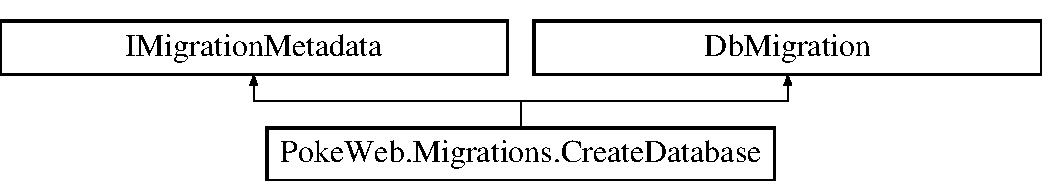
\includegraphics[height=2.000000cm]{class_poke_web_1_1_migrations_1_1_create_database}
\end{center}
\end{figure}
\subsection*{Public Member Functions}
\begin{DoxyCompactItemize}
\item 
override void \mbox{\hyperlink{class_poke_web_1_1_migrations_1_1_create_database_a1cc4a85b9c4fd02e5fc0203416de5e72}{Up}} ()
\item 
override void \mbox{\hyperlink{class_poke_web_1_1_migrations_1_1_create_database_aec9c293cc9c1ab106df22ee035171bad}{Down}} ()
\end{DoxyCompactItemize}


\subsection{Detailed Description}
Class to create/update database. This class was created for the \char`\"{}add-\/migrations\char`\"{} command in the Package Manager Console after deployment and generated the database flow to create and/or update the database structure. At each project update this command must be executed and a new \char`\"{}\+Db\+Migration\char`\"{} is created. 

\subsection{Member Function Documentation}
\mbox{\Hypertarget{class_poke_web_1_1_migrations_1_1_create_database_aec9c293cc9c1ab106df22ee035171bad}\label{class_poke_web_1_1_migrations_1_1_create_database_aec9c293cc9c1ab106df22ee035171bad}} 
\index{Poke\+Web\+::\+Migrations\+::\+Create\+Database@{Poke\+Web\+::\+Migrations\+::\+Create\+Database}!Down@{Down}}
\index{Down@{Down}!Poke\+Web\+::\+Migrations\+::\+Create\+Database@{Poke\+Web\+::\+Migrations\+::\+Create\+Database}}
\subsubsection{\texorpdfstring{Down()}{Down()}}
{\footnotesize\ttfamily override void Poke\+Web.\+Migrations.\+Create\+Database.\+Down (\begin{DoxyParamCaption}{ }\end{DoxyParamCaption})\hspace{0.3cm}{\ttfamily [inline]}}

Routine to delete tables. This routine is responsible for delete the tables in the database, mirroring the most recent structure of the objects in the project. \mbox{\Hypertarget{class_poke_web_1_1_migrations_1_1_create_database_a1cc4a85b9c4fd02e5fc0203416de5e72}\label{class_poke_web_1_1_migrations_1_1_create_database_a1cc4a85b9c4fd02e5fc0203416de5e72}} 
\index{Poke\+Web\+::\+Migrations\+::\+Create\+Database@{Poke\+Web\+::\+Migrations\+::\+Create\+Database}!Up@{Up}}
\index{Up@{Up}!Poke\+Web\+::\+Migrations\+::\+Create\+Database@{Poke\+Web\+::\+Migrations\+::\+Create\+Database}}
\subsubsection{\texorpdfstring{Up()}{Up()}}
{\footnotesize\ttfamily override void Poke\+Web.\+Migrations.\+Create\+Database.\+Up (\begin{DoxyParamCaption}{ }\end{DoxyParamCaption})\hspace{0.3cm}{\ttfamily [inline]}}

Routine to create tables. This routine is responsible for creating or updating the tables in the database, mirroring the most recent structure of the objects in the project. 

The documentation for this class was generated from the following files\+:\begin{DoxyCompactItemize}
\item 
Migrations/201801261158053\+\_\+\+Create\+Database.\+cs\item 
Migrations/201801261158053\+\_\+\+Create\+Database.\+Designer.\+cs\end{DoxyCompactItemize}

\hypertarget{class_poke_web_1_1_models_1_1_move}{}\section{Poke\+Web.\+Models.\+Move Class Reference}
\label{class_poke_web_1_1_models_1_1_move}\index{Poke\+Web.\+Models.\+Move@{Poke\+Web.\+Models.\+Move}}
\subsection*{Properties}
\begin{DoxyCompactItemize}
\item 
long \mbox{\hyperlink{class_poke_web_1_1_models_1_1_move_a3095d605c6c2a3f9e466f3d03592e4bd}{id}}\hspace{0.3cm}{\ttfamily  \mbox{[}get, set\mbox{]}}
\item 
string \mbox{\hyperlink{class_poke_web_1_1_models_1_1_move_a78bbe5e25915a5edc31479c696e80274}{name}}\hspace{0.3cm}{\ttfamily  \mbox{[}get, set\mbox{]}}
\end{DoxyCompactItemize}


\subsection{Detailed Description}
\mbox{\hyperlink{class_poke_web_1_1_models_1_1_move}{Move}} class represents the \mbox{\hyperlink{class_poke_web_1_1_models_1_1_pokemon}{Pokemon}} move object. This object is grouped in list form and related to a \mbox{\hyperlink{class_poke_web_1_1_models_1_1_pokemon}{Pokemon}} 

\subsection{Property Documentation}
\mbox{\Hypertarget{class_poke_web_1_1_models_1_1_move_a3095d605c6c2a3f9e466f3d03592e4bd}\label{class_poke_web_1_1_models_1_1_move_a3095d605c6c2a3f9e466f3d03592e4bd}} 
\index{Poke\+Web\+::\+Models\+::\+Move@{Poke\+Web\+::\+Models\+::\+Move}!id@{id}}
\index{id@{id}!Poke\+Web\+::\+Models\+::\+Move@{Poke\+Web\+::\+Models\+::\+Move}}
\subsubsection{\texorpdfstring{id}{id}}
{\footnotesize\ttfamily long Poke\+Web.\+Models.\+Move.\+id\hspace{0.3cm}{\ttfamily [get]}, {\ttfamily [set]}}

An identification element. \mbox{\Hypertarget{class_poke_web_1_1_models_1_1_move_a78bbe5e25915a5edc31479c696e80274}\label{class_poke_web_1_1_models_1_1_move_a78bbe5e25915a5edc31479c696e80274}} 
\index{Poke\+Web\+::\+Models\+::\+Move@{Poke\+Web\+::\+Models\+::\+Move}!name@{name}}
\index{name@{name}!Poke\+Web\+::\+Models\+::\+Move@{Poke\+Web\+::\+Models\+::\+Move}}
\subsubsection{\texorpdfstring{name}{name}}
{\footnotesize\ttfamily string Poke\+Web.\+Models.\+Move.\+name\hspace{0.3cm}{\ttfamily [get]}, {\ttfamily [set]}}

A name of ability. 

The documentation for this class was generated from the following file\+:\begin{DoxyCompactItemize}
\item 
Models/Move.\+cs\end{DoxyCompactItemize}

\hypertarget{class_poke_web_1_1_models_1_1_pokemon}{}\section{Poke\+Web.\+Models.\+Pokemon Class Reference}
\label{class_poke_web_1_1_models_1_1_pokemon}\index{Poke\+Web.\+Models.\+Pokemon@{Poke\+Web.\+Models.\+Pokemon}}
\subsection*{Properties}
\begin{DoxyCompactItemize}
\item 
long \mbox{\hyperlink{class_poke_web_1_1_models_1_1_pokemon_a35354c2b166053864d0faa1e3409b195}{id}}\hspace{0.3cm}{\ttfamily  \mbox{[}get, set\mbox{]}}
\item 
string \mbox{\hyperlink{class_poke_web_1_1_models_1_1_pokemon_a1ecc395a836db96ccd1f3a03006d8ec0}{name}}\hspace{0.3cm}{\ttfamily  \mbox{[}get, set\mbox{]}}
\item 
string \mbox{\hyperlink{class_poke_web_1_1_models_1_1_pokemon_a057ea49079a54039e937909cd988ca6b}{image}}\hspace{0.3cm}{\ttfamily  \mbox{[}get, set\mbox{]}}
\item 
int \mbox{\hyperlink{class_poke_web_1_1_models_1_1_pokemon_a2ae5e08e7eb16ffb86763a91e106afe4}{speed}}\hspace{0.3cm}{\ttfamily  \mbox{[}get, set\mbox{]}}
\item 
int \mbox{\hyperlink{class_poke_web_1_1_models_1_1_pokemon_aad557ec06fa783140a59b9aab7cf85a6}{defense}}\hspace{0.3cm}{\ttfamily  \mbox{[}get, set\mbox{]}}
\item 
int \mbox{\hyperlink{class_poke_web_1_1_models_1_1_pokemon_a48b57f219aaf1a924b1ecb0a64ab2f3f}{attack}}\hspace{0.3cm}{\ttfamily  \mbox{[}get, set\mbox{]}}
\item 
int \mbox{\hyperlink{class_poke_web_1_1_models_1_1_pokemon_aa0cb2ccf7bc83dd3bf65f54d7d9c760e}{special\+\_\+defense}}\hspace{0.3cm}{\ttfamily  \mbox{[}get, set\mbox{]}}
\item 
int \mbox{\hyperlink{class_poke_web_1_1_models_1_1_pokemon_a963dba983b3db5098c52716042d82ff8}{special\+\_\+attack}}\hspace{0.3cm}{\ttfamily  \mbox{[}get, set\mbox{]}}
\item 
int \mbox{\hyperlink{class_poke_web_1_1_models_1_1_pokemon_a122936a5bf25b4f565012b7daff5e577}{hp}}\hspace{0.3cm}{\ttfamily  \mbox{[}get, set\mbox{]}}
\item 
int \mbox{\hyperlink{class_poke_web_1_1_models_1_1_pokemon_ac5434e65eceb31787ee551c31f4a24ce}{base\+\_\+experience}}\hspace{0.3cm}{\ttfamily  \mbox{[}get, set\mbox{]}}
\item 
int \mbox{\hyperlink{class_poke_web_1_1_models_1_1_pokemon_a451a02460c6c35837e8d3994533e2f17}{height}}\hspace{0.3cm}{\ttfamily  \mbox{[}get, set\mbox{]}}
\item 
int \mbox{\hyperlink{class_poke_web_1_1_models_1_1_pokemon_ac0f8886171f4dc0ccab04017831f8942}{weigh}}\hspace{0.3cm}{\ttfamily  \mbox{[}get, set\mbox{]}}
\item 
virtual I\+Collection$<$ \mbox{\hyperlink{class_poke_web_1_1_models_1_1_move}{Move}} $>$ \mbox{\hyperlink{class_poke_web_1_1_models_1_1_pokemon_ad0debd8b8a90cdac3f17f6dd6d001c59}{moves}}\hspace{0.3cm}{\ttfamily  \mbox{[}get, set\mbox{]}}
\item 
virtual I\+Collection$<$ \mbox{\hyperlink{class_poke_web_1_1_models_1_1_ability}{Ability}} $>$ \mbox{\hyperlink{class_poke_web_1_1_models_1_1_pokemon_a3bb33ec8bbbe99286112d6f32c3cc96b}{abilities}}\hspace{0.3cm}{\ttfamily  \mbox{[}get, set\mbox{]}}
\end{DoxyCompactItemize}


\subsection{Detailed Description}
\mbox{\hyperlink{class_poke_web_1_1_models_1_1_pokemon}{Pokemon}} class represents the \mbox{\hyperlink{class_poke_web_1_1_models_1_1_pokemon}{Pokemon}} in all project. This object contain all information about the \mbox{\hyperlink{class_poke_web_1_1_models_1_1_pokemon}{Pokemon}} 

\subsection{Property Documentation}
\mbox{\Hypertarget{class_poke_web_1_1_models_1_1_pokemon_a3bb33ec8bbbe99286112d6f32c3cc96b}\label{class_poke_web_1_1_models_1_1_pokemon_a3bb33ec8bbbe99286112d6f32c3cc96b}} 
\index{Poke\+Web\+::\+Models\+::\+Pokemon@{Poke\+Web\+::\+Models\+::\+Pokemon}!abilities@{abilities}}
\index{abilities@{abilities}!Poke\+Web\+::\+Models\+::\+Pokemon@{Poke\+Web\+::\+Models\+::\+Pokemon}}
\subsubsection{\texorpdfstring{abilities}{abilities}}
{\footnotesize\ttfamily virtual I\+Collection$<$\mbox{\hyperlink{class_poke_web_1_1_models_1_1_ability}{Ability}}$>$ Poke\+Web.\+Models.\+Pokemon.\+abilities\hspace{0.3cm}{\ttfamily [get]}, {\ttfamily [set]}}

A list of abilities of the \mbox{\hyperlink{class_poke_web_1_1_models_1_1_pokemon}{Pokemon}}. \mbox{\Hypertarget{class_poke_web_1_1_models_1_1_pokemon_a48b57f219aaf1a924b1ecb0a64ab2f3f}\label{class_poke_web_1_1_models_1_1_pokemon_a48b57f219aaf1a924b1ecb0a64ab2f3f}} 
\index{Poke\+Web\+::\+Models\+::\+Pokemon@{Poke\+Web\+::\+Models\+::\+Pokemon}!attack@{attack}}
\index{attack@{attack}!Poke\+Web\+::\+Models\+::\+Pokemon@{Poke\+Web\+::\+Models\+::\+Pokemon}}
\subsubsection{\texorpdfstring{attack}{attack}}
{\footnotesize\ttfamily int Poke\+Web.\+Models.\+Pokemon.\+attack\hspace{0.3cm}{\ttfamily [get]}, {\ttfamily [set]}}

A attack attribute of the \mbox{\hyperlink{class_poke_web_1_1_models_1_1_pokemon}{Pokemon}}. \mbox{\Hypertarget{class_poke_web_1_1_models_1_1_pokemon_ac5434e65eceb31787ee551c31f4a24ce}\label{class_poke_web_1_1_models_1_1_pokemon_ac5434e65eceb31787ee551c31f4a24ce}} 
\index{Poke\+Web\+::\+Models\+::\+Pokemon@{Poke\+Web\+::\+Models\+::\+Pokemon}!base\+\_\+experience@{base\+\_\+experience}}
\index{base\+\_\+experience@{base\+\_\+experience}!Poke\+Web\+::\+Models\+::\+Pokemon@{Poke\+Web\+::\+Models\+::\+Pokemon}}
\subsubsection{\texorpdfstring{base\+\_\+experience}{base\_experience}}
{\footnotesize\ttfamily int Poke\+Web.\+Models.\+Pokemon.\+base\+\_\+experience\hspace{0.3cm}{\ttfamily [get]}, {\ttfamily [set]}}

A experience points attribute of the \mbox{\hyperlink{class_poke_web_1_1_models_1_1_pokemon}{Pokemon}}. \mbox{\Hypertarget{class_poke_web_1_1_models_1_1_pokemon_aad557ec06fa783140a59b9aab7cf85a6}\label{class_poke_web_1_1_models_1_1_pokemon_aad557ec06fa783140a59b9aab7cf85a6}} 
\index{Poke\+Web\+::\+Models\+::\+Pokemon@{Poke\+Web\+::\+Models\+::\+Pokemon}!defense@{defense}}
\index{defense@{defense}!Poke\+Web\+::\+Models\+::\+Pokemon@{Poke\+Web\+::\+Models\+::\+Pokemon}}
\subsubsection{\texorpdfstring{defense}{defense}}
{\footnotesize\ttfamily int Poke\+Web.\+Models.\+Pokemon.\+defense\hspace{0.3cm}{\ttfamily [get]}, {\ttfamily [set]}}

A defence attribute of the \mbox{\hyperlink{class_poke_web_1_1_models_1_1_pokemon}{Pokemon}}. \mbox{\Hypertarget{class_poke_web_1_1_models_1_1_pokemon_a451a02460c6c35837e8d3994533e2f17}\label{class_poke_web_1_1_models_1_1_pokemon_a451a02460c6c35837e8d3994533e2f17}} 
\index{Poke\+Web\+::\+Models\+::\+Pokemon@{Poke\+Web\+::\+Models\+::\+Pokemon}!height@{height}}
\index{height@{height}!Poke\+Web\+::\+Models\+::\+Pokemon@{Poke\+Web\+::\+Models\+::\+Pokemon}}
\subsubsection{\texorpdfstring{height}{height}}
{\footnotesize\ttfamily int Poke\+Web.\+Models.\+Pokemon.\+height\hspace{0.3cm}{\ttfamily [get]}, {\ttfamily [set]}}

A height attribute of the \mbox{\hyperlink{class_poke_web_1_1_models_1_1_pokemon}{Pokemon}}. \mbox{\Hypertarget{class_poke_web_1_1_models_1_1_pokemon_a122936a5bf25b4f565012b7daff5e577}\label{class_poke_web_1_1_models_1_1_pokemon_a122936a5bf25b4f565012b7daff5e577}} 
\index{Poke\+Web\+::\+Models\+::\+Pokemon@{Poke\+Web\+::\+Models\+::\+Pokemon}!hp@{hp}}
\index{hp@{hp}!Poke\+Web\+::\+Models\+::\+Pokemon@{Poke\+Web\+::\+Models\+::\+Pokemon}}
\subsubsection{\texorpdfstring{hp}{hp}}
{\footnotesize\ttfamily int Poke\+Web.\+Models.\+Pokemon.\+hp\hspace{0.3cm}{\ttfamily [get]}, {\ttfamily [set]}}

A health points attribute of the \mbox{\hyperlink{class_poke_web_1_1_models_1_1_pokemon}{Pokemon}}. \mbox{\Hypertarget{class_poke_web_1_1_models_1_1_pokemon_a35354c2b166053864d0faa1e3409b195}\label{class_poke_web_1_1_models_1_1_pokemon_a35354c2b166053864d0faa1e3409b195}} 
\index{Poke\+Web\+::\+Models\+::\+Pokemon@{Poke\+Web\+::\+Models\+::\+Pokemon}!id@{id}}
\index{id@{id}!Poke\+Web\+::\+Models\+::\+Pokemon@{Poke\+Web\+::\+Models\+::\+Pokemon}}
\subsubsection{\texorpdfstring{id}{id}}
{\footnotesize\ttfamily long Poke\+Web.\+Models.\+Pokemon.\+id\hspace{0.3cm}{\ttfamily [get]}, {\ttfamily [set]}}

An identification element. \mbox{\Hypertarget{class_poke_web_1_1_models_1_1_pokemon_a057ea49079a54039e937909cd988ca6b}\label{class_poke_web_1_1_models_1_1_pokemon_a057ea49079a54039e937909cd988ca6b}} 
\index{Poke\+Web\+::\+Models\+::\+Pokemon@{Poke\+Web\+::\+Models\+::\+Pokemon}!image@{image}}
\index{image@{image}!Poke\+Web\+::\+Models\+::\+Pokemon@{Poke\+Web\+::\+Models\+::\+Pokemon}}
\subsubsection{\texorpdfstring{image}{image}}
{\footnotesize\ttfamily string Poke\+Web.\+Models.\+Pokemon.\+image\hspace{0.3cm}{\ttfamily [get]}, {\ttfamily [set]}}

A path to \mbox{\hyperlink{class_poke_web_1_1_models_1_1_pokemon}{Pokemon}} image. \mbox{\Hypertarget{class_poke_web_1_1_models_1_1_pokemon_ad0debd8b8a90cdac3f17f6dd6d001c59}\label{class_poke_web_1_1_models_1_1_pokemon_ad0debd8b8a90cdac3f17f6dd6d001c59}} 
\index{Poke\+Web\+::\+Models\+::\+Pokemon@{Poke\+Web\+::\+Models\+::\+Pokemon}!moves@{moves}}
\index{moves@{moves}!Poke\+Web\+::\+Models\+::\+Pokemon@{Poke\+Web\+::\+Models\+::\+Pokemon}}
\subsubsection{\texorpdfstring{moves}{moves}}
{\footnotesize\ttfamily virtual I\+Collection$<$\mbox{\hyperlink{class_poke_web_1_1_models_1_1_move}{Move}}$>$ Poke\+Web.\+Models.\+Pokemon.\+moves\hspace{0.3cm}{\ttfamily [get]}, {\ttfamily [set]}}

A list of moves of the \mbox{\hyperlink{class_poke_web_1_1_models_1_1_pokemon}{Pokemon}}. \mbox{\Hypertarget{class_poke_web_1_1_models_1_1_pokemon_a1ecc395a836db96ccd1f3a03006d8ec0}\label{class_poke_web_1_1_models_1_1_pokemon_a1ecc395a836db96ccd1f3a03006d8ec0}} 
\index{Poke\+Web\+::\+Models\+::\+Pokemon@{Poke\+Web\+::\+Models\+::\+Pokemon}!name@{name}}
\index{name@{name}!Poke\+Web\+::\+Models\+::\+Pokemon@{Poke\+Web\+::\+Models\+::\+Pokemon}}
\subsubsection{\texorpdfstring{name}{name}}
{\footnotesize\ttfamily string Poke\+Web.\+Models.\+Pokemon.\+name\hspace{0.3cm}{\ttfamily [get]}, {\ttfamily [set]}}

A name of \mbox{\hyperlink{class_poke_web_1_1_models_1_1_pokemon}{Pokemon}}. \mbox{\Hypertarget{class_poke_web_1_1_models_1_1_pokemon_a963dba983b3db5098c52716042d82ff8}\label{class_poke_web_1_1_models_1_1_pokemon_a963dba983b3db5098c52716042d82ff8}} 
\index{Poke\+Web\+::\+Models\+::\+Pokemon@{Poke\+Web\+::\+Models\+::\+Pokemon}!special\+\_\+attack@{special\+\_\+attack}}
\index{special\+\_\+attack@{special\+\_\+attack}!Poke\+Web\+::\+Models\+::\+Pokemon@{Poke\+Web\+::\+Models\+::\+Pokemon}}
\subsubsection{\texorpdfstring{special\+\_\+attack}{special\_attack}}
{\footnotesize\ttfamily int Poke\+Web.\+Models.\+Pokemon.\+special\+\_\+attack\hspace{0.3cm}{\ttfamily [get]}, {\ttfamily [set]}}

A special attack attribute of the \mbox{\hyperlink{class_poke_web_1_1_models_1_1_pokemon}{Pokemon}}. \mbox{\Hypertarget{class_poke_web_1_1_models_1_1_pokemon_aa0cb2ccf7bc83dd3bf65f54d7d9c760e}\label{class_poke_web_1_1_models_1_1_pokemon_aa0cb2ccf7bc83dd3bf65f54d7d9c760e}} 
\index{Poke\+Web\+::\+Models\+::\+Pokemon@{Poke\+Web\+::\+Models\+::\+Pokemon}!special\+\_\+defense@{special\+\_\+defense}}
\index{special\+\_\+defense@{special\+\_\+defense}!Poke\+Web\+::\+Models\+::\+Pokemon@{Poke\+Web\+::\+Models\+::\+Pokemon}}
\subsubsection{\texorpdfstring{special\+\_\+defense}{special\_defense}}
{\footnotesize\ttfamily int Poke\+Web.\+Models.\+Pokemon.\+special\+\_\+defense\hspace{0.3cm}{\ttfamily [get]}, {\ttfamily [set]}}

A special defence attribute of the \mbox{\hyperlink{class_poke_web_1_1_models_1_1_pokemon}{Pokemon}}. \mbox{\Hypertarget{class_poke_web_1_1_models_1_1_pokemon_a2ae5e08e7eb16ffb86763a91e106afe4}\label{class_poke_web_1_1_models_1_1_pokemon_a2ae5e08e7eb16ffb86763a91e106afe4}} 
\index{Poke\+Web\+::\+Models\+::\+Pokemon@{Poke\+Web\+::\+Models\+::\+Pokemon}!speed@{speed}}
\index{speed@{speed}!Poke\+Web\+::\+Models\+::\+Pokemon@{Poke\+Web\+::\+Models\+::\+Pokemon}}
\subsubsection{\texorpdfstring{speed}{speed}}
{\footnotesize\ttfamily int Poke\+Web.\+Models.\+Pokemon.\+speed\hspace{0.3cm}{\ttfamily [get]}, {\ttfamily [set]}}

A speed attribute of the \mbox{\hyperlink{class_poke_web_1_1_models_1_1_pokemon}{Pokemon}}. \mbox{\Hypertarget{class_poke_web_1_1_models_1_1_pokemon_ac0f8886171f4dc0ccab04017831f8942}\label{class_poke_web_1_1_models_1_1_pokemon_ac0f8886171f4dc0ccab04017831f8942}} 
\index{Poke\+Web\+::\+Models\+::\+Pokemon@{Poke\+Web\+::\+Models\+::\+Pokemon}!weigh@{weigh}}
\index{weigh@{weigh}!Poke\+Web\+::\+Models\+::\+Pokemon@{Poke\+Web\+::\+Models\+::\+Pokemon}}
\subsubsection{\texorpdfstring{weigh}{weigh}}
{\footnotesize\ttfamily int Poke\+Web.\+Models.\+Pokemon.\+weigh\hspace{0.3cm}{\ttfamily [get]}, {\ttfamily [set]}}

A weigh attribute of the \mbox{\hyperlink{class_poke_web_1_1_models_1_1_pokemon}{Pokemon}}. 

The documentation for this class was generated from the following file\+:\begin{DoxyCompactItemize}
\item 
Models/Pokemon.\+cs\end{DoxyCompactItemize}

\hypertarget{class_poke_web_1_1_controllers_1_1pokemon_controller}{}\section{Poke\+Web.\+Controllers.\+pokemon\+Controller Class Reference}
\label{class_poke_web_1_1_controllers_1_1pokemon_controller}\index{Poke\+Web.\+Controllers.\+pokemon\+Controller@{Poke\+Web.\+Controllers.\+pokemon\+Controller}}
Inheritance diagram for Poke\+Web.\+Controllers.\+pokemon\+Controller\+:\begin{figure}[H]
\begin{center}
\leavevmode
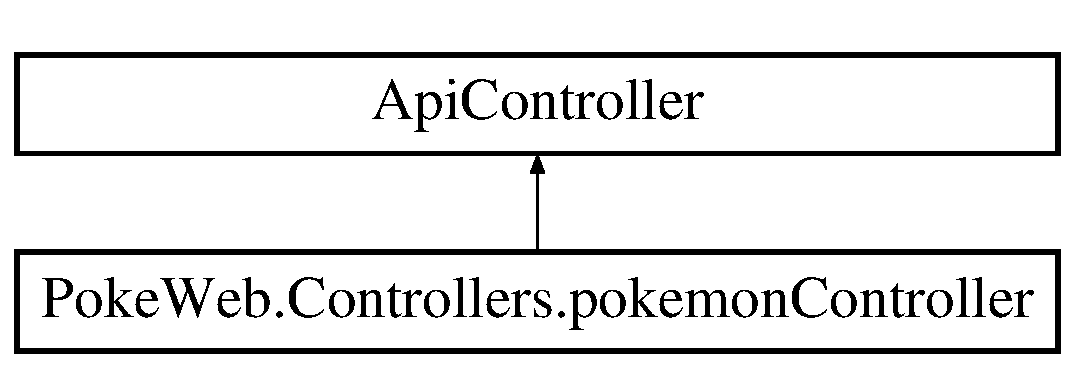
\includegraphics[height=2.000000cm]{class_poke_web_1_1_controllers_1_1pokemon_controller}
\end{center}
\end{figure}
\subsection*{Public Member Functions}
\begin{DoxyCompactItemize}
\item 
I\+Http\+Action\+Result \mbox{\hyperlink{class_poke_web_1_1_controllers_1_1pokemon_controller_a5d8946d4d1cbf4cb9b044ef2e7cb7492}{Get\+All\+Pokemons}} (int page\+\_\+size, int page)
\item 
I\+Http\+Action\+Result \mbox{\hyperlink{class_poke_web_1_1_controllers_1_1pokemon_controller_a631a03b01ec3e0b99e9751c2f9def3bb}{Get\+First6\+Pokemons\+Order\+By\+Atack\+Desc}} ()
\item 
I\+Http\+Action\+Result \mbox{\hyperlink{class_poke_web_1_1_controllers_1_1pokemon_controller_a31ee4aa642842e5fb9a2c1ceaf42f0b6}{Get\+Pokemon}} (int id)
\item 
I\+Http\+Action\+Result \mbox{\hyperlink{class_poke_web_1_1_controllers_1_1pokemon_controller_a426f7fbc4f620f8f7b6f144f10233540}{Post\+Pokemon}} (\mbox{\hyperlink{class_poke_web_1_1_models_1_1_pokemon}{Pokemon}} pokemon)
\item 
I\+Http\+Action\+Result \mbox{\hyperlink{class_poke_web_1_1_controllers_1_1pokemon_controller_a155329861c4235adf1e8ebf27c3fa19e}{Put\+Pokemon}} (\mbox{\hyperlink{class_poke_web_1_1_models_1_1_pokemon}{Pokemon}} pokemon)
\item 
I\+Http\+Action\+Result \mbox{\hyperlink{class_poke_web_1_1_controllers_1_1pokemon_controller_a563cc501f839af2bf76b57b8a8c26dd0}{Patch\+Pokemon}} (\mbox{\hyperlink{class_poke_web_1_1_models_1_1_pokemon}{Pokemon}} pokemon)
\item 
I\+Http\+Action\+Result \mbox{\hyperlink{class_poke_web_1_1_controllers_1_1pokemon_controller_a8ba6862493be8003dc42bebe58578da4}{Delete\+Pokemon}} (int id)
\end{DoxyCompactItemize}


\subsection{Detailed Description}
Primary controller of the A\+PI application. This controller is responsible for receiving all requests in the application and handling each of the calls according to the route and parameters received. 

\subsection{Member Function Documentation}
\mbox{\Hypertarget{class_poke_web_1_1_controllers_1_1pokemon_controller_a8ba6862493be8003dc42bebe58578da4}\label{class_poke_web_1_1_controllers_1_1pokemon_controller_a8ba6862493be8003dc42bebe58578da4}} 
\index{Poke\+Web\+::\+Controllers\+::pokemon\+Controller@{Poke\+Web\+::\+Controllers\+::pokemon\+Controller}!Delete\+Pokemon@{Delete\+Pokemon}}
\index{Delete\+Pokemon@{Delete\+Pokemon}!Poke\+Web\+::\+Controllers\+::pokemon\+Controller@{Poke\+Web\+::\+Controllers\+::pokemon\+Controller}}
\subsubsection{\texorpdfstring{Delete\+Pokemon()}{DeletePokemon()}}
{\footnotesize\ttfamily I\+Http\+Action\+Result Poke\+Web.\+Controllers.\+pokemon\+Controller.\+Delete\+Pokemon (\begin{DoxyParamCaption}\item[{int}]{id }\end{DoxyParamCaption})\hspace{0.3cm}{\ttfamily [inline]}}

Routine to delete a Pokemon. This routine is responsible for remove data about the Pokemon into the application with identification


\begin{DoxyParams}{Parameters}
{\em Pokemon} & Identification of Pokemon in database \\
\hline
\end{DoxyParams}
\begin{DoxyReturn}{Returns}
Data of Pokemon removed 
\end{DoxyReturn}
\begin{DoxyAuthor}{Author}
Rafael M. S. Siqueira 
\end{DoxyAuthor}
\mbox{\Hypertarget{class_poke_web_1_1_controllers_1_1pokemon_controller_a5d8946d4d1cbf4cb9b044ef2e7cb7492}\label{class_poke_web_1_1_controllers_1_1pokemon_controller_a5d8946d4d1cbf4cb9b044ef2e7cb7492}} 
\index{Poke\+Web\+::\+Controllers\+::pokemon\+Controller@{Poke\+Web\+::\+Controllers\+::pokemon\+Controller}!Get\+All\+Pokemons@{Get\+All\+Pokemons}}
\index{Get\+All\+Pokemons@{Get\+All\+Pokemons}!Poke\+Web\+::\+Controllers\+::pokemon\+Controller@{Poke\+Web\+::\+Controllers\+::pokemon\+Controller}}
\subsubsection{\texorpdfstring{Get\+All\+Pokemons()}{GetAllPokemons()}}
{\footnotesize\ttfamily I\+Http\+Action\+Result Poke\+Web.\+Controllers.\+pokemon\+Controller.\+Get\+All\+Pokemons (\begin{DoxyParamCaption}\item[{int}]{page\+\_\+size,  }\item[{int}]{page }\end{DoxyParamCaption})\hspace{0.3cm}{\ttfamily [inline]}}

Routine for Pokemon listings. This routine operates by paging system, facilitating the client-\/side iplementation. To be executed, this routine waits for two parameters, the page size (number of elements returned) and the page number.


\begin{DoxyParams}{Parameters}
{\em page\+\_\+size} & Number of elements \\
\hline
{\em page} & Number of page \\
\hline
\end{DoxyParams}
\begin{DoxyReturn}{Returns}
List of Pokemons 
\end{DoxyReturn}
\begin{DoxyAuthor}{Author}
Rafael M. S. Siqueira 
\end{DoxyAuthor}
\mbox{\Hypertarget{class_poke_web_1_1_controllers_1_1pokemon_controller_a631a03b01ec3e0b99e9751c2f9def3bb}\label{class_poke_web_1_1_controllers_1_1pokemon_controller_a631a03b01ec3e0b99e9751c2f9def3bb}} 
\index{Poke\+Web\+::\+Controllers\+::pokemon\+Controller@{Poke\+Web\+::\+Controllers\+::pokemon\+Controller}!Get\+First6\+Pokemons\+Order\+By\+Atack\+Desc@{Get\+First6\+Pokemons\+Order\+By\+Atack\+Desc}}
\index{Get\+First6\+Pokemons\+Order\+By\+Atack\+Desc@{Get\+First6\+Pokemons\+Order\+By\+Atack\+Desc}!Poke\+Web\+::\+Controllers\+::pokemon\+Controller@{Poke\+Web\+::\+Controllers\+::pokemon\+Controller}}
\subsubsection{\texorpdfstring{Get\+First6\+Pokemons\+Order\+By\+Atack\+Desc()}{GetFirst6PokemonsOrderByAtackDesc()}}
{\footnotesize\ttfamily I\+Http\+Action\+Result Poke\+Web.\+Controllers.\+pokemon\+Controller.\+Get\+First6\+Pokemons\+Order\+By\+Atack\+Desc (\begin{DoxyParamCaption}{ }\end{DoxyParamCaption})\hspace{0.3cm}{\ttfamily [inline]}}

Routine for the list of 6 best Pokemons ordered by attack points. This routine lists the 6 best pokémons ordered by the attack parameter and calculates the statistical data for this group to help the client about this information.

\begin{DoxyReturn}{Returns}
Container with the list of 6 top Pokemons ans statistic data 
\end{DoxyReturn}
\begin{DoxyAuthor}{Author}
Rafael M. S. Siqueira 
\end{DoxyAuthor}
\mbox{\Hypertarget{class_poke_web_1_1_controllers_1_1pokemon_controller_a31ee4aa642842e5fb9a2c1ceaf42f0b6}\label{class_poke_web_1_1_controllers_1_1pokemon_controller_a31ee4aa642842e5fb9a2c1ceaf42f0b6}} 
\index{Poke\+Web\+::\+Controllers\+::pokemon\+Controller@{Poke\+Web\+::\+Controllers\+::pokemon\+Controller}!Get\+Pokemon@{Get\+Pokemon}}
\index{Get\+Pokemon@{Get\+Pokemon}!Poke\+Web\+::\+Controllers\+::pokemon\+Controller@{Poke\+Web\+::\+Controllers\+::pokemon\+Controller}}
\subsubsection{\texorpdfstring{Get\+Pokemon()}{GetPokemon()}}
{\footnotesize\ttfamily I\+Http\+Action\+Result Poke\+Web.\+Controllers.\+pokemon\+Controller.\+Get\+Pokemon (\begin{DoxyParamCaption}\item[{int}]{id }\end{DoxyParamCaption})\hspace{0.3cm}{\ttfamily [inline]}}

Routine for Pokemon details. This Pokemon gets the identification number of a Pokemon and returns all the data in the application related to that Pokemon


\begin{DoxyParams}{Parameters}
{\em id} & Identification of Pokemon in database \\
\hline
\end{DoxyParams}
\begin{DoxyReturn}{Returns}
Data of Pokemon 
\end{DoxyReturn}
\begin{DoxyAuthor}{Author}
Rafael M. S. Siqueira 
\end{DoxyAuthor}
\mbox{\Hypertarget{class_poke_web_1_1_controllers_1_1pokemon_controller_a563cc501f839af2bf76b57b8a8c26dd0}\label{class_poke_web_1_1_controllers_1_1pokemon_controller_a563cc501f839af2bf76b57b8a8c26dd0}} 
\index{Poke\+Web\+::\+Controllers\+::pokemon\+Controller@{Poke\+Web\+::\+Controllers\+::pokemon\+Controller}!Patch\+Pokemon@{Patch\+Pokemon}}
\index{Patch\+Pokemon@{Patch\+Pokemon}!Poke\+Web\+::\+Controllers\+::pokemon\+Controller@{Poke\+Web\+::\+Controllers\+::pokemon\+Controller}}
\subsubsection{\texorpdfstring{Patch\+Pokemon()}{PatchPokemon()}}
{\footnotesize\ttfamily I\+Http\+Action\+Result Poke\+Web.\+Controllers.\+pokemon\+Controller.\+Patch\+Pokemon (\begin{DoxyParamCaption}\item[{\mbox{\hyperlink{class_poke_web_1_1_models_1_1_pokemon}{Pokemon}}}]{pokemon }\end{DoxyParamCaption})\hspace{0.3cm}{\ttfamily [inline]}}

Routine to send a Pokemon. This routine is responsible for update a part of infromation about the Pokemon into the application in database


\begin{DoxyParams}{Parameters}
{\em Pokemon} & Part of infoirmation about the Pokemon \\
\hline
\end{DoxyParams}
\begin{DoxyReturn}{Returns}
Data of Pokemon with identification 
\end{DoxyReturn}
\begin{DoxyAuthor}{Author}
Rafael M. S. Siqueira 
\end{DoxyAuthor}
\mbox{\Hypertarget{class_poke_web_1_1_controllers_1_1pokemon_controller_a426f7fbc4f620f8f7b6f144f10233540}\label{class_poke_web_1_1_controllers_1_1pokemon_controller_a426f7fbc4f620f8f7b6f144f10233540}} 
\index{Poke\+Web\+::\+Controllers\+::pokemon\+Controller@{Poke\+Web\+::\+Controllers\+::pokemon\+Controller}!Post\+Pokemon@{Post\+Pokemon}}
\index{Post\+Pokemon@{Post\+Pokemon}!Poke\+Web\+::\+Controllers\+::pokemon\+Controller@{Poke\+Web\+::\+Controllers\+::pokemon\+Controller}}
\subsubsection{\texorpdfstring{Post\+Pokemon()}{PostPokemon()}}
{\footnotesize\ttfamily I\+Http\+Action\+Result Poke\+Web.\+Controllers.\+pokemon\+Controller.\+Post\+Pokemon (\begin{DoxyParamCaption}\item[{\mbox{\hyperlink{class_poke_web_1_1_models_1_1_pokemon}{Pokemon}}}]{pokemon }\end{DoxyParamCaption})\hspace{0.3cm}{\ttfamily [inline]}}

Routine to send a Pokemon. This routine is responsible for inserting a Pokemon into the application or updating all the data if it is already registered in the database of the application


\begin{DoxyParams}{Parameters}
{\em Pokemon} & All infoirmation about the Pokemon \\
\hline
\end{DoxyParams}
\begin{DoxyReturn}{Returns}
Data of Pokemon with identification 
\end{DoxyReturn}
\begin{DoxyAuthor}{Author}
Rafael M. S. Siqueira 
\end{DoxyAuthor}
\mbox{\Hypertarget{class_poke_web_1_1_controllers_1_1pokemon_controller_a155329861c4235adf1e8ebf27c3fa19e}\label{class_poke_web_1_1_controllers_1_1pokemon_controller_a155329861c4235adf1e8ebf27c3fa19e}} 
\index{Poke\+Web\+::\+Controllers\+::pokemon\+Controller@{Poke\+Web\+::\+Controllers\+::pokemon\+Controller}!Put\+Pokemon@{Put\+Pokemon}}
\index{Put\+Pokemon@{Put\+Pokemon}!Poke\+Web\+::\+Controllers\+::pokemon\+Controller@{Poke\+Web\+::\+Controllers\+::pokemon\+Controller}}
\subsubsection{\texorpdfstring{Put\+Pokemon()}{PutPokemon()}}
{\footnotesize\ttfamily I\+Http\+Action\+Result Poke\+Web.\+Controllers.\+pokemon\+Controller.\+Put\+Pokemon (\begin{DoxyParamCaption}\item[{\mbox{\hyperlink{class_poke_web_1_1_models_1_1_pokemon}{Pokemon}}}]{pokemon }\end{DoxyParamCaption})\hspace{0.3cm}{\ttfamily [inline]}}

Routine to send a Pokemon. This routine is responsible for inserting a Pokemon into the application all the data if it is already registered in the database of the application


\begin{DoxyParams}{Parameters}
{\em Pokemon} & All infoirmation about the Pokemon \\
\hline
\end{DoxyParams}
\begin{DoxyReturn}{Returns}
Data of Pokemon with identification 
\end{DoxyReturn}
\begin{DoxyAuthor}{Author}
Rafael M. S. Siqueira 
\end{DoxyAuthor}


The documentation for this class was generated from the following file\+:\begin{DoxyCompactItemize}
\item 
Controllers/pokemon\+Controller.\+cs\end{DoxyCompactItemize}

\hypertarget{class_poke_web_1_1_d_a_l_1_1_poke_web_context}{}\section{Poke\+Web.\+D\+A\+L.\+Poke\+Web\+Context Class Reference}
\label{class_poke_web_1_1_d_a_l_1_1_poke_web_context}\index{Poke\+Web.\+D\+A\+L.\+Poke\+Web\+Context@{Poke\+Web.\+D\+A\+L.\+Poke\+Web\+Context}}
Inheritance diagram for Poke\+Web.\+D\+A\+L.\+Poke\+Web\+Context\+:\begin{figure}[H]
\begin{center}
\leavevmode
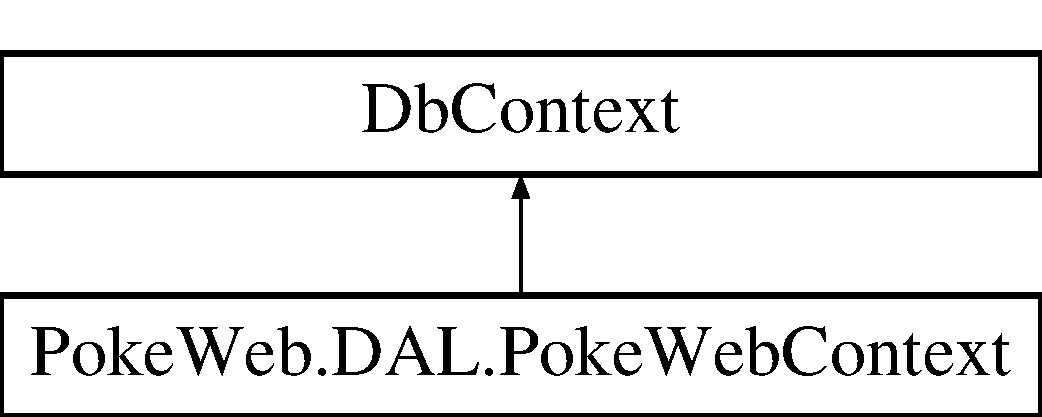
\includegraphics[height=2.000000cm]{class_poke_web_1_1_d_a_l_1_1_poke_web_context}
\end{center}
\end{figure}
\subsection*{Public Member Functions}
\begin{DoxyCompactItemize}
\item 
\mbox{\hyperlink{class_poke_web_1_1_d_a_l_1_1_poke_web_context_ad657dbdf7487f5fb5c13fde61726fe3d}{Poke\+Web\+Context}} ()
\end{DoxyCompactItemize}
\subsection*{Properties}
\begin{DoxyCompactItemize}
\item 
Db\+Set$<$ \mbox{\hyperlink{class_poke_web_1_1_models_1_1_pokemon}{Models.\+Pokemon}} $>$ \mbox{\hyperlink{class_poke_web_1_1_d_a_l_1_1_poke_web_context_ac3e453f7ae2467d1910a0db7e074dc93}{Pokemons}}\hspace{0.3cm}{\ttfamily  \mbox{[}get, set\mbox{]}}
\end{DoxyCompactItemize}


\subsection{Detailed Description}
Class of context database. This class is user for Entity\+Framework an extend \char`\"{}\+Db\+Context\char`\"{} to manage the access of database with My\+S\+QL Server 2014. 

\subsection{Constructor \& Destructor Documentation}
\mbox{\Hypertarget{class_poke_web_1_1_d_a_l_1_1_poke_web_context_ad657dbdf7487f5fb5c13fde61726fe3d}\label{class_poke_web_1_1_d_a_l_1_1_poke_web_context_ad657dbdf7487f5fb5c13fde61726fe3d}} 
\index{Poke\+Web\+::\+D\+A\+L\+::\+Poke\+Web\+Context@{Poke\+Web\+::\+D\+A\+L\+::\+Poke\+Web\+Context}!Poke\+Web\+Context@{Poke\+Web\+Context}}
\index{Poke\+Web\+Context@{Poke\+Web\+Context}!Poke\+Web\+::\+D\+A\+L\+::\+Poke\+Web\+Context@{Poke\+Web\+::\+D\+A\+L\+::\+Poke\+Web\+Context}}
\subsubsection{\texorpdfstring{Poke\+Web\+Context()}{PokeWebContext()}}
{\footnotesize\ttfamily Poke\+Web.\+D\+A\+L.\+Poke\+Web\+Context.\+Poke\+Web\+Context (\begin{DoxyParamCaption}{ }\end{DoxyParamCaption})\hspace{0.3cm}{\ttfamily [inline]}}

Constructor of database context. This contriuctor mapping access data informatio this T\+AG \char`\"{}\+Poke\+Web\+Context\char`\"{} in \char`\"{}\+Web.\+config\char`\"{} file. 

\subsection{Property Documentation}
\mbox{\Hypertarget{class_poke_web_1_1_d_a_l_1_1_poke_web_context_ac3e453f7ae2467d1910a0db7e074dc93}\label{class_poke_web_1_1_d_a_l_1_1_poke_web_context_ac3e453f7ae2467d1910a0db7e074dc93}} 
\index{Poke\+Web\+::\+D\+A\+L\+::\+Poke\+Web\+Context@{Poke\+Web\+::\+D\+A\+L\+::\+Poke\+Web\+Context}!Pokemons@{Pokemons}}
\index{Pokemons@{Pokemons}!Poke\+Web\+::\+D\+A\+L\+::\+Poke\+Web\+Context@{Poke\+Web\+::\+D\+A\+L\+::\+Poke\+Web\+Context}}
\subsubsection{\texorpdfstring{Pokemons}{Pokemons}}
{\footnotesize\ttfamily Db\+Set$<$\mbox{\hyperlink{class_poke_web_1_1_models_1_1_pokemon}{Models.\+Pokemon}}$>$ Poke\+Web.\+D\+A\+L.\+Poke\+Web\+Context.\+Pokemons\hspace{0.3cm}{\ttfamily [get]}, {\ttfamily [set]}}

Dataset to map object Pokemon in database. This used with Entity Framework to generate all resources with percistence using My\+S\+QL Server 2014. 

The documentation for this class was generated from the following file\+:\begin{DoxyCompactItemize}
\item 
D\+A\+L/Poke\+Web\+Context.\+cs\end{DoxyCompactItemize}

\hypertarget{class_poke_web_1_1_models_1_1_statistic}{}\section{Poke\+Web.\+Models.\+Statistic Class Reference}
\label{class_poke_web_1_1_models_1_1_statistic}\index{Poke\+Web.\+Models.\+Statistic@{Poke\+Web.\+Models.\+Statistic}}
\subsection*{Properties}
\begin{DoxyCompactItemize}
\item 
int \mbox{\hyperlink{class_poke_web_1_1_models_1_1_statistic_adde59f67e6296c8557f35cefb422da34}{speed}}\hspace{0.3cm}{\ttfamily  \mbox{[}get, set\mbox{]}}
\item 
int \mbox{\hyperlink{class_poke_web_1_1_models_1_1_statistic_a16b525d351bdddcced3a66fbb695a7de}{defense}}\hspace{0.3cm}{\ttfamily  \mbox{[}get, set\mbox{]}}
\item 
int \mbox{\hyperlink{class_poke_web_1_1_models_1_1_statistic_abbb2828f554117e55eef4cb42f0cf315}{attack}}\hspace{0.3cm}{\ttfamily  \mbox{[}get, set\mbox{]}}
\item 
int \mbox{\hyperlink{class_poke_web_1_1_models_1_1_statistic_a0bab71d5765c664af820349a3bd3ebfd}{special\+\_\+defense}}\hspace{0.3cm}{\ttfamily  \mbox{[}get, set\mbox{]}}
\item 
int \mbox{\hyperlink{class_poke_web_1_1_models_1_1_statistic_af02035e2eb7d45f5ecb79743ff96a765}{special\+\_\+attack}}\hspace{0.3cm}{\ttfamily  \mbox{[}get, set\mbox{]}}
\item 
int \mbox{\hyperlink{class_poke_web_1_1_models_1_1_statistic_a27c55b3b5ef9ab129af79eff794664b1}{hp}}\hspace{0.3cm}{\ttfamily  \mbox{[}get, set\mbox{]}}
\end{DoxyCompactItemize}


\subsection{Detailed Description}
\mbox{\hyperlink{class_poke_web_1_1_models_1_1_statistic}{Statistic}} class represents the \mbox{\hyperlink{class_poke_web_1_1_models_1_1_pokemon}{Pokemon}} sum attributes. This object is created where clint request the 6 top attacks points Pokemons 

\subsection{Property Documentation}
\mbox{\Hypertarget{class_poke_web_1_1_models_1_1_statistic_abbb2828f554117e55eef4cb42f0cf315}\label{class_poke_web_1_1_models_1_1_statistic_abbb2828f554117e55eef4cb42f0cf315}} 
\index{Poke\+Web\+::\+Models\+::\+Statistic@{Poke\+Web\+::\+Models\+::\+Statistic}!attack@{attack}}
\index{attack@{attack}!Poke\+Web\+::\+Models\+::\+Statistic@{Poke\+Web\+::\+Models\+::\+Statistic}}
\subsubsection{\texorpdfstring{attack}{attack}}
{\footnotesize\ttfamily int Poke\+Web.\+Models.\+Statistic.\+attack\hspace{0.3cm}{\ttfamily [get]}, {\ttfamily [set]}}

A attack attribute sum of the \mbox{\hyperlink{class_poke_web_1_1_models_1_1_pokemon}{Pokemon}}. \mbox{\Hypertarget{class_poke_web_1_1_models_1_1_statistic_a16b525d351bdddcced3a66fbb695a7de}\label{class_poke_web_1_1_models_1_1_statistic_a16b525d351bdddcced3a66fbb695a7de}} 
\index{Poke\+Web\+::\+Models\+::\+Statistic@{Poke\+Web\+::\+Models\+::\+Statistic}!defense@{defense}}
\index{defense@{defense}!Poke\+Web\+::\+Models\+::\+Statistic@{Poke\+Web\+::\+Models\+::\+Statistic}}
\subsubsection{\texorpdfstring{defense}{defense}}
{\footnotesize\ttfamily int Poke\+Web.\+Models.\+Statistic.\+defense\hspace{0.3cm}{\ttfamily [get]}, {\ttfamily [set]}}

A defence attribute sum of the \mbox{\hyperlink{class_poke_web_1_1_models_1_1_pokemon}{Pokemon}}. \mbox{\Hypertarget{class_poke_web_1_1_models_1_1_statistic_a27c55b3b5ef9ab129af79eff794664b1}\label{class_poke_web_1_1_models_1_1_statistic_a27c55b3b5ef9ab129af79eff794664b1}} 
\index{Poke\+Web\+::\+Models\+::\+Statistic@{Poke\+Web\+::\+Models\+::\+Statistic}!hp@{hp}}
\index{hp@{hp}!Poke\+Web\+::\+Models\+::\+Statistic@{Poke\+Web\+::\+Models\+::\+Statistic}}
\subsubsection{\texorpdfstring{hp}{hp}}
{\footnotesize\ttfamily int Poke\+Web.\+Models.\+Statistic.\+hp\hspace{0.3cm}{\ttfamily [get]}, {\ttfamily [set]}}

A speed health points sum of the \mbox{\hyperlink{class_poke_web_1_1_models_1_1_pokemon}{Pokemon}}. \mbox{\Hypertarget{class_poke_web_1_1_models_1_1_statistic_af02035e2eb7d45f5ecb79743ff96a765}\label{class_poke_web_1_1_models_1_1_statistic_af02035e2eb7d45f5ecb79743ff96a765}} 
\index{Poke\+Web\+::\+Models\+::\+Statistic@{Poke\+Web\+::\+Models\+::\+Statistic}!special\+\_\+attack@{special\+\_\+attack}}
\index{special\+\_\+attack@{special\+\_\+attack}!Poke\+Web\+::\+Models\+::\+Statistic@{Poke\+Web\+::\+Models\+::\+Statistic}}
\subsubsection{\texorpdfstring{special\+\_\+attack}{special\_attack}}
{\footnotesize\ttfamily int Poke\+Web.\+Models.\+Statistic.\+special\+\_\+attack\hspace{0.3cm}{\ttfamily [get]}, {\ttfamily [set]}}

A special attack attribute sum of the \mbox{\hyperlink{class_poke_web_1_1_models_1_1_pokemon}{Pokemon}}. \mbox{\Hypertarget{class_poke_web_1_1_models_1_1_statistic_a0bab71d5765c664af820349a3bd3ebfd}\label{class_poke_web_1_1_models_1_1_statistic_a0bab71d5765c664af820349a3bd3ebfd}} 
\index{Poke\+Web\+::\+Models\+::\+Statistic@{Poke\+Web\+::\+Models\+::\+Statistic}!special\+\_\+defense@{special\+\_\+defense}}
\index{special\+\_\+defense@{special\+\_\+defense}!Poke\+Web\+::\+Models\+::\+Statistic@{Poke\+Web\+::\+Models\+::\+Statistic}}
\subsubsection{\texorpdfstring{special\+\_\+defense}{special\_defense}}
{\footnotesize\ttfamily int Poke\+Web.\+Models.\+Statistic.\+special\+\_\+defense\hspace{0.3cm}{\ttfamily [get]}, {\ttfamily [set]}}

A special defence attribute sum of the \mbox{\hyperlink{class_poke_web_1_1_models_1_1_pokemon}{Pokemon}}. \mbox{\Hypertarget{class_poke_web_1_1_models_1_1_statistic_adde59f67e6296c8557f35cefb422da34}\label{class_poke_web_1_1_models_1_1_statistic_adde59f67e6296c8557f35cefb422da34}} 
\index{Poke\+Web\+::\+Models\+::\+Statistic@{Poke\+Web\+::\+Models\+::\+Statistic}!speed@{speed}}
\index{speed@{speed}!Poke\+Web\+::\+Models\+::\+Statistic@{Poke\+Web\+::\+Models\+::\+Statistic}}
\subsubsection{\texorpdfstring{speed}{speed}}
{\footnotesize\ttfamily int Poke\+Web.\+Models.\+Statistic.\+speed\hspace{0.3cm}{\ttfamily [get]}, {\ttfamily [set]}}

A speed attribute sum of the \mbox{\hyperlink{class_poke_web_1_1_models_1_1_pokemon}{Pokemon}}. 

The documentation for this class was generated from the following file\+:\begin{DoxyCompactItemize}
\item 
Models/Statistic.\+cs\end{DoxyCompactItemize}

\hypertarget{class_poke_web_1_1_models_1_1_statistic_container}{}\section{Poke\+Web.\+Models.\+Statistic\+Container Class Reference}
\label{class_poke_web_1_1_models_1_1_statistic_container}\index{Poke\+Web.\+Models.\+Statistic\+Container@{Poke\+Web.\+Models.\+Statistic\+Container}}
\subsection*{Properties}
\begin{DoxyCompactItemize}
\item 
I\+List$<$ \mbox{\hyperlink{class_poke_web_1_1_models_1_1_pokemon}{Pokemon}} $>$ \mbox{\hyperlink{class_poke_web_1_1_models_1_1_statistic_container_a6604be3f919e9d1f389f78f844438c54}{pokemons}}\hspace{0.3cm}{\ttfamily  \mbox{[}get, set\mbox{]}}
\item 
\mbox{\hyperlink{class_poke_web_1_1_models_1_1_statistic}{Statistic}} \mbox{\hyperlink{class_poke_web_1_1_models_1_1_statistic_container_a4d3cb3c4061cd7077870bcd1675aaff6}{statistic}}\hspace{0.3cm}{\ttfamily  \mbox{[}get, set\mbox{]}}
\end{DoxyCompactItemize}


\subsection{Detailed Description}
\mbox{\hyperlink{class_poke_web_1_1_models_1_1_statistic_container}{Statistic\+Container}} class represents the list of top 6 Pokemons and statistics data. This object is created where clint request the 6 top attacks points Pokemons and used to return de statistic data and the list of top 6 Pokemons 

\subsection{Property Documentation}
\mbox{\Hypertarget{class_poke_web_1_1_models_1_1_statistic_container_a6604be3f919e9d1f389f78f844438c54}\label{class_poke_web_1_1_models_1_1_statistic_container_a6604be3f919e9d1f389f78f844438c54}} 
\index{Poke\+Web\+::\+Models\+::\+Statistic\+Container@{Poke\+Web\+::\+Models\+::\+Statistic\+Container}!pokemons@{pokemons}}
\index{pokemons@{pokemons}!Poke\+Web\+::\+Models\+::\+Statistic\+Container@{Poke\+Web\+::\+Models\+::\+Statistic\+Container}}
\subsubsection{\texorpdfstring{pokemons}{pokemons}}
{\footnotesize\ttfamily I\+List$<$\mbox{\hyperlink{class_poke_web_1_1_models_1_1_pokemon}{Pokemon}}$>$ Poke\+Web.\+Models.\+Statistic\+Container.\+pokemons\hspace{0.3cm}{\ttfamily [get]}, {\ttfamily [set]}}

List of 6 top attack attribute Pokemons \mbox{\Hypertarget{class_poke_web_1_1_models_1_1_statistic_container_a4d3cb3c4061cd7077870bcd1675aaff6}\label{class_poke_web_1_1_models_1_1_statistic_container_a4d3cb3c4061cd7077870bcd1675aaff6}} 
\index{Poke\+Web\+::\+Models\+::\+Statistic\+Container@{Poke\+Web\+::\+Models\+::\+Statistic\+Container}!statistic@{statistic}}
\index{statistic@{statistic}!Poke\+Web\+::\+Models\+::\+Statistic\+Container@{Poke\+Web\+::\+Models\+::\+Statistic\+Container}}
\subsubsection{\texorpdfstring{statistic}{statistic}}
{\footnotesize\ttfamily \mbox{\hyperlink{class_poke_web_1_1_models_1_1_statistic}{Statistic}} Poke\+Web.\+Models.\+Statistic\+Container.\+statistic\hspace{0.3cm}{\ttfamily [get]}, {\ttfamily [set]}}

\mbox{\hyperlink{class_poke_web_1_1_models_1_1_statistic}{Statistic}} data about this goup of Pokemons 

The documentation for this class was generated from the following file\+:\begin{DoxyCompactItemize}
\item 
Models/Statistic.\+cs\end{DoxyCompactItemize}

\hypertarget{class_poke_web_1_1_swagger_config}{}\section{Poke\+Web.\+Swagger\+Config Class Reference}
\label{class_poke_web_1_1_swagger_config}\index{Poke\+Web.\+Swagger\+Config@{Poke\+Web.\+Swagger\+Config}}
\subsection*{Static Public Member Functions}
\begin{DoxyCompactItemize}
\item 
\mbox{\Hypertarget{class_poke_web_1_1_swagger_config_a518fcb5f0f0675bda318488e3919db72}\label{class_poke_web_1_1_swagger_config_a518fcb5f0f0675bda318488e3919db72}} 
static void {\bfseries Register} ()
\end{DoxyCompactItemize}


The documentation for this class was generated from the following file\+:\begin{DoxyCompactItemize}
\item 
App\+\_\+\+Start/Swagger\+Config.\+cs\end{DoxyCompactItemize}

\hypertarget{class_poke_web_1_1_web_api_application}{}\section{Poke\+Web.\+Web\+Api\+Application Class Reference}
\label{class_poke_web_1_1_web_api_application}\index{Poke\+Web.\+Web\+Api\+Application@{Poke\+Web.\+Web\+Api\+Application}}
Inheritance diagram for Poke\+Web.\+Web\+Api\+Application\+:\begin{figure}[H]
\begin{center}
\leavevmode
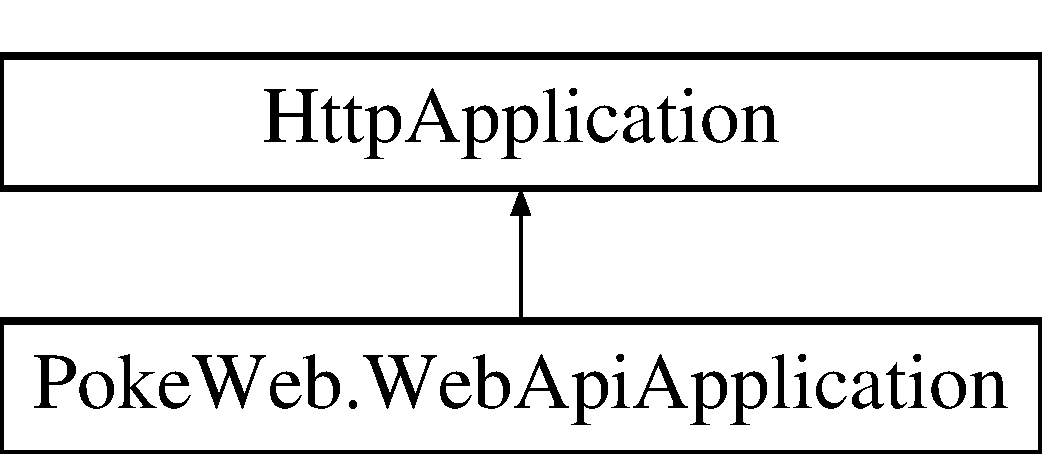
\includegraphics[height=2.000000cm]{class_poke_web_1_1_web_api_application}
\end{center}
\end{figure}
\subsection*{Protected Member Functions}
\begin{DoxyCompactItemize}
\item 
\mbox{\Hypertarget{class_poke_web_1_1_web_api_application_a63a50d86f7dd6e9417238218fe90cdb2}\label{class_poke_web_1_1_web_api_application_a63a50d86f7dd6e9417238218fe90cdb2}} 
void {\bfseries Application\+\_\+\+Start} ()
\end{DoxyCompactItemize}


The documentation for this class was generated from the following file\+:\begin{DoxyCompactItemize}
\item 
Global.\+asax.\+cs\end{DoxyCompactItemize}

%--- End generated contents ---

% Index
\backmatter
\newpage
\phantomsection
\clearemptydoublepage
\addcontentsline{toc}{chapter}{Index}
\printindex

\end{document}
